\chapter{Variabili Aleatorie Indipendenti}
Dal concetto di indipendenza tra \emph{eventi} discende naturalmente quello di 
\emph{indipendenza tra variabili aleatorie}, che rappresenta la condizione in cui le variabili considerate non si influenzano reciprocamente. 
Introdurremo diversi criteri utili a stabilire formalmente l’indipendenza, alcuni dei quali permetteranno di apprezzare il ruolo del valore atteso 
oltre la semplice interpretazione come indicatore numerico. 

\medskip
\noindent Mostreremo inoltre come sia possibile costruire variabili aleatorie indipendenti a partire da variabili arbitrarie, 
e come tale proprietà consenta di estendere la teoria precedente ai \emph{prodotti cartesiani} tra domini, dando origine alle corrispondenti $\sigma$--algebre prodotto e alle relative misure di probabilità. 

\medskip
\noindent Tale struttura consentirà di introdurre le \emph{leggi congiunte}, ottenute a partire dalle \emph{leggi marginali} mediante l’applicazione 
del fondamentale \emph{teorema di Fubini--Tonelli}. Questo ci condurrà infine verso lo studio dei \emph{vettori aleatori}, ossia variabili aleatorie a valori multidimensionali, che rappresentano il naturale passo successivo nell’analisi delle relazioni stocastiche tra più componenti casuali.

\section{Variabili Aleatorie Unidimensionali}
Immaginiamo quindi di avere uno stesso esperimento dal quale si osservano due o più grandezze.\\
Avremo quindi uno stesso spazio di probabilità $(\Omega, \mathcal{A}, \mathbb{P})$ sul quale sono definite due variabili aleatorie:
\begin{align*}
    X:(\Omega, \mathcal{A}, \mathbb{P})\to (F_1, \mathcal{F}_1)\\
    Y:(\Omega, \mathcal{A}, \mathbb{P})\to (F_2, \mathcal{F}_2)
\end{align*}

Vogliamo quindi studiare quale sia la relazione tra $X$ ed $Y$.

\begin{definizione}
    Dato $(\Omega, \mathcal{A}, \mathbb{P})$ e $(F_1, \mathcal{F}_1), \; (F_2, \mathcal{F}_2)\;$ spazi misurabili, e le variabili aleatorie 
    \begin{align*}
    X:(\Omega, \mathcal{A}, \mathbb{P})\to (F_1, \mathcal{F}_1)\\
    Y:(\Omega, \mathcal{A}, \mathbb{P})\to (F_2, \mathcal{F}_2)
\end{align*}
Allora $X$ ed $Y$ sono indipendenti se:
\[\forall A\in\mathcal{F}_1, \;\forall B\in\mathcal{F}_2\;\text{ si ha che: }\qquad \mathbb{P}\big((X\in A)\cap (Y\in B)\big) = \mathbb{P}(X\in A)\cdot \mathbb{P}(Y\in B)\]
\end{definizione}

\begin{proposizione}
    Si ha che:
    \[X\ind Y\qquad\iff\qquad \sigma(X)\ind \sigma(Y)\]\footnotetext{Si ricorda la Definizione \ref{def:3.13}}
\end{proposizione}

\begin{esempio}
    Si immagini di avere un contenitore con $N$ palline nere e $B$ palline bianche; si estragga con reimmissione una pallina per $k$ volte.\\
    Possiamo definire $X_k = \begin{cases}
        1, \quad &\text{se $k$--esima estrazione esce nera}\\
        0, & \text{altrimenti}
    \end{cases}$

    \medskip
    \noindent Ci chiediamo, $X_1$ e $X_2$ sono indipendenti?\\
    \\
    Si noti innanzitutto che $\Omega= \{B, N\}\times\{B, N\}$, e che dato $(w_1, w_2)\in\Omega$ allora conosciamo tutte le probabilità degli eventi $\mathbb{P}(\{B, N\}) = \frac{BN}{(B+N)^2},\; \mathbb{P}(\{B, B\}) ...$.\\
    Devo verificare che sia valido che
    \[\mathbb{P}\big((X_1\in A)\cap (X_2\in B)\big) = \mathbb{P}(X_1\in A)\cdot \mathbb{P}(X_2\in B)\]
    dove \[A, B\in2^{\{0, 1\}} = \set{\{0\}, \{1\}, \{0, 1\}, \varnothing} = \sigma(\{1\})\]
    Ipotizzando che $A=B=\{1\}, \;$ allora avremo che:
     \[\mathbb{P}\big((X_1=1)\cap (X_2=1)\big) = \mathbb{P}(\{N, N\}) = \frac{N}{N+B} \frac{N}{N+B} = \mathbb{P}({X_1=1})\cdot\mathbb{P}(X_2 = 1)\qquad \checkmark\]

    Ipotizzando che $A=B=\{0\}, \;$ allora avremo che:
     \[\mathbb{P}\big((X_1=0)\cap (X_2=0)\big) = \mathbb{P}(\{B, B\}) = \frac{B}{N+B} \frac{B}{N+B} = \mathbb{P}({X_1=0})\cdot\mathbb{P}(X_2 = 0)\qquad \checkmark\]

     Posso quindi controllare solo che le controimmagini siano indipendenti per concludere che lo siano tutti gli eventi appartenenti alle $\sigma$--algebre delle 
     V.A.
\end{esempio}

\begin{teorema}[Condizioni Equivalenti all'Indipendenza]
\label{th:condind}
    Siano $(\Omega, \mathcal{A}, \mathbb{P}), (F_1, \mathcal{F}_1),  (F_2, \mathcal{F}_2)$ assegnati, e siano $X_1:\Omega\to F_1$ e $X_2:\Omega\to F_2$ variabili aleatorie.\\
    Sono equivalenti le seguenti:
    \begin{enumerate}
        \item $\boxed{X\ind Y}$
        \item Date $\;h:(F_1, \mathcal{F}_1)\to (E_1, \mathcal{E}_1),\;$ e $ \; g:(F_2, \mathcal{F}_2)\to(E_2, \mathcal{E}_2)$ \[\boxed{h(X)\ind g(Y)}\]
        \item $\forall h:F_1\to \mathbb{R}\;\text{ e }\; \forall g:F_2\to \mathbb{R}\;$ entrambe non negative o limitate $\quad \Rightarrow\quad h(X), g(Y)$ ammettono valore atteso e:
        \[\boxed{E\left[h(X)\cdot g(Y)\right] = E\left[h(X)\right]\cdot E\left[g(Y)\right]}\]
        \item $\forall h\in L^1(F_1, \mathcal{F}_1, P^X)\;\text{ e }\;\forall g\in L^1(F_2, \mathcal{F}_2, P^Y)$
        \[\boxed{E\left[h(X)\cdot g(Y)\right] = E\left[h(X)\right]\cdot E\left[g(Y)\right] = \int_{F_1}h(x)\;dP^X \cdot \int_{F_2}g(y)\;dP^Y}\]
    \end{enumerate}
\end{teorema}

\noindent Inoltre, applicando quello che già sappiamo dai capitoli precedenti:
\[\begin{aligned}
    \forall h\in L^1(F_1, \mathcal{F}_1, P^X)\\
    \forall g\in L^1(F_2, \mathcal{F}_2, P^Y)
\end{aligned} \qquad \iff \qquad \int_{F_1}|h|\;dP^X<+\infty \quad \text{e}\quad \int_{F_2}|g|\;dP^Y<+\infty\]
e quindi:
\begin{align*}
    E\left[\left|h(X)\right|\cdot \left|g(Y)\right|\right] &=  \int_{F_1}|h|\;dP^X \cdot \int_{F_2}|g|\;dP^Y = \int_{\Omega}|h(X)|\;d\mathbb{P}\cdot\int_{\Omega}|g(Y)|\;d\mathbb{P}\\
    & = \int_\Omega |h(X)\cdot g(Y)|\;d\mathbb{P}
\end{align*}
\[\Rightarrow \qquad h(X), g(Y)\in L^1(\mathbb{P})\quad\text{ e }\quad E[h(X)\cdot g(Y)] = E[h(X)]\cdot E[g(Y)]\]

\bigskip
\noindent Possiamo riassumere ciò che abbiamo appena trovato nel seguente corollario:
\begin{corollario}
    Se $X, Y\in L^1(\Omega, \mathcal{A}, \mathbb{P})$ e vale che $X\ind Y$:
    \[\Rightarrow\qquad X\cdot Y \in L^1 \quad \text{e}\quad E[XY] = E[X]E[Y]\]

    \begin{dimostrazione}
        Dal Teorema \ref{th:condind}.4, con $h, g = \text{Id}$:
        \begin{align*}
            X\in L^1(\mathbb{P})\quad &\iff \quad \text{Id} \in L^1(P^X)\\
            Y\in L^1(\mathbb{P})\quad &\iff \quad \text{Id} \in L^1(P^Y)
        \end{align*}
        Essendo indipendenti:
        \[E[h(X)\cdot g(Y)] = E[X\cdot Y] = E[X] \cdot E[Y]\]
    \end{dimostrazione}
\end{corollario}

Osserviamo che dal Teorema \ref{th:condind}.2 possiamo ricavare che se $X\ind Y$ e $X=W$ quasi certamente, allora avrò che $W \ind Y$.

\section{Variabili Aleatorie Multidimensionali: Sigme--Algebre Prodotto}
Abbiamo visto l'indipendenza tra variabili aleatorie, ma potremmo estendere il ragionamento ai vettori.

\medskip 
\noindent Date quindi due variabili aleatorie, costruiamo il vettore che ha per componenti le due V.A.
\[\begin{aligned}
    & X: (\Omega, \mathcal{A}, \mathbb{P})\to (F_1, \mathcal{F}_1)\\
    & Y: (\Omega, \mathcal{A}, \mathbb{P})\to (F_2, \mathcal{F}_2)
\end{aligned} \qquad\Longrightarrow\qquad
\begin{pmatrix} X\\Y \end{pmatrix} :(\Omega, \mathcal{A}, \mathbb{P})\to (F_1 \times F_2, ??)\]

\noindent A questo punto ci chiediamo:

\begin{itemize}
    \item Questo è una variabile aleatoria come vettore?
    \item La legge congiunta $P^{(X, Y)}$ dove è definita nel caso?
\end{itemize}

\bigskip
\noindent È evidente che tutta la questione può essere ridotta alla seguente domanda: \textit{Dati $F_1, F_2$ e facendone il prodotto cartesiano $F = F_1\times F_2$, quale è la $\sigma$--algebra ``naturale'' di questo nuovo dominio $F$?}

\medskip
A prima vista potrebbe sembrare logico prendere $\mathcal{F}_1\times \mathcal{F}_2$ come $\sigma$--algebra di definizione dello spazio di arrivo; questo però non è possibile, in quanto $\mathcal{F}_1\times \mathcal{F}_2$ \textbf{non è} una $\sigma$--algebra.
\[\mathcal{F}_1\times \mathcal{F}_2 = \set{C\subseteq F_1\times F_2:\;C = A\times B,\quad A\in \mathcal{F}_1, \;B\in \mathcal{F}_2}\]

\noindent Questo risulta evidente già nel caso semplice in cui $F_1 = F_2 = \mathbb{R}$. Difatti, presi come da figura $A_1, B_1 \in \mathcal{F}_1$ e $A_2, B_2\in \mathcal{F}_2$, possiamo costruire gli insiemi prodotto $A = A_1\times A_2$ e $B = B_1\times B_2$.

\begin{figure}[H]
\centering
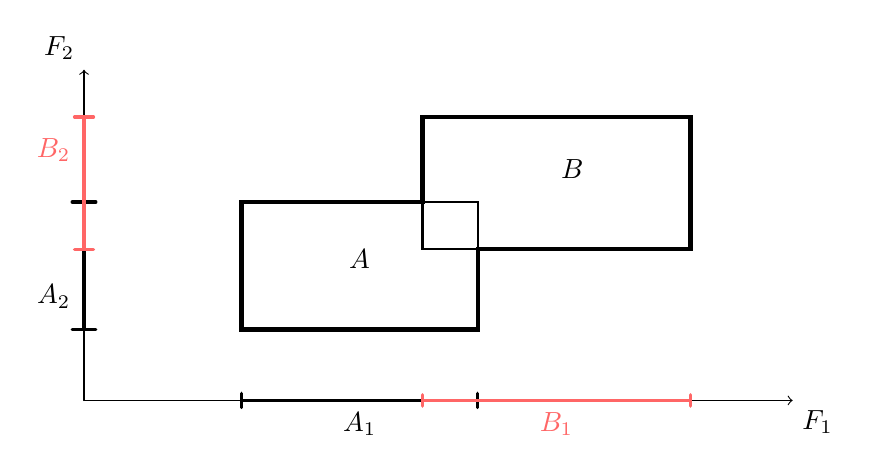
\begin{tikzpicture}[x=1cm,y=0.6cm,line cap=round]

% --- Assi ---
\draw[ thin,->] (0,0) -- (9,0) node[below right] {$F_1$};
\draw[ thin,->] (0,0) -- (0,7) node[above left]  {$F_2$};

% --- Tacche e etichette su Omega_1 ---
\draw[very thick] (2,-0.15)--(2,0.15);
\draw[very thick] (5,-0.15)--(5,0.15);
\draw[very thick] (2, 0)--(5, 0);
\draw[very thick, red!60] (4.3, 0)--(7.7, 0);
\node[below] at (3.5,-0.05) {$A_1$};
\draw[red!60,very thick] (4.3,-0.12)--(4.3,0.12);
\draw[red!60,very thick] (7.7,-0.12)--(7.7,0.12);
\node[red!60,below] at (6,-0.05) {$B_1$};

% --- Tacche e etichette su Omega_2 ---
\draw[very thick] (-0.15,1.5)--(0.15,1.5);
\draw[very thick] (-0.15,4.2)--(0.15,4.2);
\draw[very thick] (0,1.5)--(0,4.2);
\draw[very thick, red!60] (0,3.2)--(0, 6);
\node[left] at (-0.05,2.2) {$A_2$};
\draw[red!60,very thick] (-0.12,3.2)--(0.12,3.2);
\draw[red!60,very thick] (-0.12,6)--(0.12,6);
\node[red!60,left] at (-0.05,5.3) {$B_2$};

% --- Rettangolo A ---
\draw[ thick] (2,1.5) rectangle (5,4.2);
\node at (3.5,3.0) {$A$};

% --- Rettangolo B ---
\draw[ thick] (4.3,3.2) rectangle (7.7,6.0);
\node at (6.2,4.9) {$B$};

\draw[ultra thick]
  (2,1.5) -- (2,4.2) -- (4.3,4.2) -- (4.3,6.0) --
  (7.7,6.0) -- (7.7,3.2) -- (5,3.2) -- (5,1.5) -- cycle;


\end{tikzpicture}
\end{figure}

È facile notare che l'intersezione $A\cap B$, può essere espressa come come prodotto cartesiano, e dunque è un sottoinsieme di $\mathcal{F}_1\times\mathcal{F}_2$:
\[A\cap B = (A_1 \cap B_1)\times (A_2\cap B_2) \in \mathcal{F}_1\times\mathcal{F}_2\]

Questo purtroppo non è possibile farlo per l'unione $A\cup B$, che anche graficamente si vede che non risulta essere un rettangolo:
\[A\cup B = (A_1\times A_2)\cup (B_1\times B_2) \notin \mathcal{F}_1\times\mathcal{F}_2\]

\noindent È quindi evidente che $\mathcal{F}_1\times\mathcal{F}_2$ non è una $\sigma$--algebra, in quanto non è chiusa per unioni (né per complementazione).\\
\\
Siamo però fortunati lo stesso: $\mathcal{F}_1\times\mathcal{F}_2$ risulta essere un $\Pi$--sistema (Teorema \ref{th:caratheodory}) per $F = F_1 \times F_2$; ecco che si risolve il problema che avevamo: possiamo finalmente definire una nuova $\sigma$--algebra sulla quale il nostro vettore $(X, Y)^\top$ risulta essere misurabile.

\begin{definizione}[Sigma--Algebra Prodotto]
    Dati $(F_1, \mathcal{F}_1), \,(F_2, \mathcal{F}_2)$ spazi misurabili si definisce $\sigma$--algebra prodotto (o prodotto tensore):
    \[\mathcal{F}_1 \otimes\mathcal{F}_2 = \sigma(\mathcal{F}_1 \times\mathcal{F}_2)\]
\end{definizione}

\noindent Possiamo rispondere ai dubbi esposti all'inizio dell sezione, definendo il vettore aleatorio sui seguenti spazi:

\[\begin{pmatrix} X\\Y \end{pmatrix} :(\Omega, \mathcal{A}, \mathbb{P})\to (F_1 \times F_2, \mathcal{F}_1 \otimes\mathcal{F}_2)\]

Posso considerare $P^{(X, Y)}$ la legge di $(X, Y)^\top$, la quale è una misura di probabilità su $(\mathcal{F}_1 \otimes\mathcal{F}_2)$. $P^X$ e $P^Y$ sono dette leggi marginali, e sono le leggi delle componenti.

\begin{teorema}
    Siano $\begin{aligned}
    & X: (\Omega, \mathcal{A}, \mathbb{P})\to (F_1, \mathcal{F}_1)\\
    & Y: (\Omega, \mathcal{A}, \mathbb{P})\to (F_2, \mathcal{F}_2)
\end{aligned}\;\text{ e sia }\;h:(F_1 \times F_2, \mathcal{F}_1 \otimes\mathcal{F}_2)\to \mathbb{R},\;$ allora valgono:
\begin{enumerate}
    \item $\mathcal{B}(\mathbb{R})\otimes \mathcal{B}(\mathbb{R}) = \mathcal{B}(\mathbb{R}^2)$. In generale: $\quad \mathcal{B}(\mathbb{R})\otimes \cdots\otimes \mathcal{B}(\mathbb{R}) = \mathcal{B}(\mathbb{R}^n)$
    \item $\begin{pmatrix} X\\Y \end{pmatrix} :(\Omega, \mathcal{A}, \mathbb{P})\to (F_1 \times F_2, \mathcal{F}_1 \otimes\mathcal{F}_2)\;$ è un vettore aleatorio
    \item Si ha che ``le sezioni sono misurabili'':
    \begin{align*}
        h(x, \cdot): (F_2, \mathcal{F}_2)&\to (\mathbb{R}, \mathcal{B}(\mathbb{R})) \qquad \forall x\in F_1\\
        h(\cdot, y): (F_1, \mathcal{F}_1)&\to (\mathbb{R}, \mathcal{B}(\mathbb{R})) \qquad \forall y\in F_2
    \end{align*}
    Dove la notazione $h(\cdot, y)$ indica che è una variabile solo di $x$, e fisso la $y$.
\end{enumerate}
\end{teorema}

\begin{esempio}
    Sia $h(x, y) = \mathbb{I}_C(x, y)\;\text{ dove }\; C = \left\{(x, y)\in\mathbb{R}^2\mid x^2+y^2=1\right\}$.\\
    Allora si ha che:
    % Sezione verticale (a x fissato): sottoinsiemi di R
\[C_x := \{y\in\mathbb{R} : (x,y)\in C\}
     = \{y\in\mathbb{R} : x^2+y^2=1\}
     =
\begin{cases}
\{\; \sqrt{1-x^2},\; -\sqrt{1-x^2}\;\}, & |x|<1,\\[2pt]
\{0\}, & |x|=1,\\[2pt]
\varnothing, & |x|>1.
\end{cases}\]

% Sezione orizzontale (a y fissato): sottoinsiemi di R
\[C_y := \{x\in\mathbb{R} : (x,y)\in C\}
     = \{x\in\mathbb{R} : x^2+y^2=1\}
     =
\begin{cases}
\{\; \sqrt{1-y^2},\; -\sqrt{1-y^2}\;\}, & |y|<1,\\[2pt]
\{0\}, & |y|=1,\\[2pt]
\varnothing, & |y|>1.
\end{cases}\]

Di conseguenza le sezioni risultano essere
    \[h(x,\cdot) = \mathbb{I}_{[\sqrt{1-x^2},\; -\sqrt{1-x^2}]}(y),\qquad h(\cdot,y) = \mathbb{I}_{[\sqrt{1-y^2},\; -\sqrt{1-y^2}\;]}(x)\]
    e quindi misurabili.
\end{esempio}

\section{Teorema di Fubini--Tonelli}


Siano $X : (\Omega,\mathcal{A},P) \to (F_1,\mathcal{F}_1)$ e 
$Y : (\Omega,\mathcal{A},P) \to (F_2,\mathcal{F}_2)$ due variabili aleatorie, e
\[
(X,Y)^\top : (\Omega,\mathcal{A},P) \longrightarrow 
(F_1\times F_2,\;\mathcal{F}_1\otimes\mathcal{F}_2)
\]
la variabile aleatoria vettoriale associata. Indichiamo con
$P^X$, $P^Y$ e $P^{(X,Y)}$ rispettivamente le leggi marginali di $X$ e $Y$ 
e la legge congiunta.

\medskip
\noindent Ci chiediamo: \textit{esiste una relazione tra le marginali e la congiunta?}\\
Senza troppi formalismi, andiamo a cercare di capire intuitivamente quale potrebbe essere. Per definizione, abbiamo che
\begin{align*}
    P^X(A) &= \mathbb{P}(X\in A),\qquad \forall A\in \mathcal{F}_1\\
    P^Y(B) &= \mathbb{P}(Y\in B),\qquad \forall B\in \mathcal{F}_2
\end{align*}
\noindent e, più in generale,
\[
P^{(X,Y)}(C) = \mathbb{P}\big((X,Y)\in C\big),
\qquad 
C\in\mathcal{F}_1\otimes\mathcal{F}_2.
\]
Pertanto, prendendo $A\in\mathcal{F}_1$ e $B\in\mathcal{F}_2$ ed ``alzandoli'', ovvero si considera $F_1\times B\subseteq F_1\times F_2$ e \\
$A\times F_2\subseteq F_1\times F_2,\;$ allora:
\begin{align*}
    P^{(X,Y)}(A\times F_2) &= \mathbb{P}(X\in A, \;Y\in F_2) = \mathbb{P}(X\in A) = P^X(A)\\
    P^{(X,Y)}(F_1\times B) &= \mathbb{P}(X\in F_1, \;Y\in B) = \mathbb{P}(Y\in B) = P^Y(B).
\end{align*}

\noindent Quindi, \textbf{a partire dalla legge congiunta, è sempre possibile ricavare le leggi marginali}.

\bigskip
\noindent \textit{Ma è vero il viceversa?}

\medskip
\noindent Siccome si ha che:
\[
P^{(X,Y)}(A\times B) = P(X\in A,\,Y\in B)
\]
\textbf{non si può dedurre la congiunta dai soli valori delle marginali} $P^X(A)$ e $P^Y(B)$.  
Le marginali descrivono i comportamenti di $X$ e $Y$ presi separatamente, 
ma non contengono informazione sulla loro dipendenza.\\
\\
Esiste un unico caso in cui è possibile ricostruire la legge congiunta a partire dalle marginali: quando $X$ e $Y$ sono indipendenti.  
In tal caso,
\[
P(X\in A,\,Y\in B) = P(X\in A)\,P(Y\in B),
\]
cioè
\[
P^{(X,Y)}(A\times B) = P^X(A)\,P^Y(B)
\qquad\forall A\in\mathcal{F}_1,\;B\in\mathcal{F}_2
\]

\bigskip
\noindent Adesso che abbiamo capito intuitivamente dove si vuole arrivare, costruiamo il tutto con una teoria solida.\\
\\
Siano $(E_1, \mathcal{E}_2), \; (E_2, \mathcal{E}_2)$ spazi misurabili, e siano $\mu_1, \mu_2$ delle misure $\sigma$--finite rispettivamente definite su $(E_1, \mathcal{E}_2), \; (E_2, \mathcal{E}_2)$. Possiamo costruire lo spazio di misura $(E_1\times E_2, \mathcal{E}_1 \otimes \mathcal{E}_2)$.\\

\noindent \textit{Esiste una misura $\mu$ su $(E_1\times E_2, \mathcal{E}_1 \otimes \mathcal{E}_2)$ tale che $\mu (A\times B) = \mu_1(A)\cdot \mu_2(B)\quad \forall A\times B \in \mathcal{E}_1\times \mathcal{E}_2$?}

\begin{teorema}[Teorema di Fubini--Tonelli]
        Siano $(E_1, \mathcal{E}_2), \; (E_2, \mathcal{E}_2)$ spazi misurabili, e siano $\mu_1, \mu_2$ delle misure $\sigma$--finite rispettivamente definite su $(E_1, \mathcal{E}_2), \; (E_2, \mathcal{E}_2)$, allora:
        \begin{enumerate}
            \item $\exists!\; \mu = \mu_1\otimes\mu_2$ detta misura prodotto definita su $(\mathcal{E}_1 \otimes \mathcal{E}_2)$ tale che:
            \[\mu(A\times B) = \mu_1\otimes\mu_2(A\times B) = \mu_1(A)\cdot \mu_2(B)\qquad \quad \begin{aligned}
                \forall A\in \mathcal{E}_1,\;\forall B\in \mathcal{E}_2\\
                \forall A\times B \in \mathcal{E}_1\times \mathcal{E}_2
            \end{aligned}\]
            \item $\forall h:(E_1\times E_2, \mathcal{E}_1 \otimes \mathcal{E}_2)\to [0, +\infty]$:
            \begin{itemize}
                \item Le seguenti mappe sono misurabili e non negative:
                \[x\longmapsto\int_{E_2} h(x, y)\;\mu_2(dy), \qquad y\longmapsto\int_{E_1}h(x, y)\;\mu_1(dx)\]
                \item Vale che:
                \[\int_{E_1\times E_2}h(x, y)\;d(\mu_1\otimes \mu_2) = \int_{E_1}\left(\int_{E_2}h(x, y)\;d\mu_2\right)d\mu_1\]
            \end{itemize}
            \item $\forall h\in L^1(E_1\times E_2, \mathcal{E}_1 \otimes \mathcal{E}_2, \mu_1\otimes\mu_2)$:
            \begin{itemize}
                \item Si ha che $\qquad \begin{aligned}
                h(x, \cdot) \in L^1(E_2, \mathcal{E}_2, \mu_2) \quad &\mu_1\text{--quasi ogni }\;x\\
                h(\cdot, y) \in L^1(E_1, \mathcal{E}_1, \mu_1) \quad &\mu_2\text{--quasi ogni }\;y 
            \end{aligned}$
            \item Le seguenti mappe sono integrabili:
            \begin{align*}
                &x\longmapsto\int_{E_2} h(x, y)\;d\mu_2\quad\in L^1(E_1, \mathcal{E}_1, \mu_1)\\
                &y\longmapsto\int_{E_1}h(x, y)\;d\mu_1 \quad \in L^1(E_2, \mathcal{E}_2, \mu_2)
            \end{align*}
            e vale che 
            \[\boxed{\int_{E_1\times E_2}h(x, y)\;d(\mu_1\otimes \mu_2) = \int_{E_1}\left(\int_{E_2}h(x, y)\;d\mu_2\right)d\mu_1 = \int_{E_2}\left(\int_{E_1}h(x, y)\;d\mu_1\right)d\mu_2}\]
            \end{itemize}
        \end{enumerate}
\end{teorema}

\noindent Possiamo notare che grazie a questo teorema importantissimo abbiamo che:
\begin{align*}
    h\in L^1 (\mu_1 \otimes \mu_2)\quad & \iff \quad \int_{E_1\times E_2}|h|\;d(\mu_1\otimes \mu_2)<+\infty\\
    &\iff \quad \int_{E_1}\left(\int_{E_2}|h|\;d\mu_2\right)d\mu_1 <+\infty
\end{align*}

\bigskip
\noindent Inoltre, il teorema è stato enunciato per misure generali $\sigma$--finite; questo vuol dire che possiamo specializzare il teorema a misure di probabilità, le quali sono misure finite.

\medskip
\noindent Si considerino $\mathbb{P}_1, \;\mathbb{P}_2$ due misure di probabilità rispettivamente su $(E_1, \mathcal{E}_1), \;(E_2, \mathcal{E}_2)$.

\[\overset{\text{F.T.}}{\Longrightarrow} \quad \exists!\; \mathbb{P}_1\otimes \mathbb{P}_2\;\text{ su }\; (E_1\times E_2, \mathcal{E}_1 \otimes \mathcal{E}_2)\qquad \text{ t.c. }\qquad \mathbb{P}_1\otimes \mathbb{P}_2(A\times B)= \mathbb{P}_1(A)\cdot \mathbb{P}_2(B)\]
e valgono tutte le altre tesi del Teorema di Fubini--Tonelli.\\
\\
Si osservi infine un fatto interessante:
\begin{itemize}
    \item Se $A = E_1 \quad \Rightarrow\quad \mathbb{P}_1\otimes\mathbb{P}_2(E_1\times B) = \mathbb{P}_1(E_1)\cdot \mathbb{P}_2(B) = \mathbb{P}_2(B)$
    \item Se $B = E_2 \quad \Rightarrow\quad \mathbb{P}_1\otimes\mathbb{P}_2(A\times E_2) = \mathbb{P}_1(A)\cdot \mathbb{P}_2(E_2) = \mathbb{P}_1(A)$
\end{itemize}

\begin{teorema}[F.T. su $\mathbb{R}^n$ con $m_n$]

Sia dato il teorema di Fubini--Tonelli su $\mathbb{R}^n$ con $m_n$.\\
Consideriamo $(\mathbb{R}^{n_1}, \mathcal{B}^{n_1}, m_{n_1}),\;(\mathbb{R}^{n_2}, \mathcal{B}^{n_2}, m_{n_2})\;\text{ e }\;\bigl(\mathbb{R}^{n_1} \times \mathbb{R}^{n_2},\, \mathcal{B}^{n_1} \otimes \mathcal{B}^{n_2}\bigr)
= \bigl(\mathbb{R}^{n_1+n_2},\, \mathcal{B}^{n_1+n_2}\bigr)$.\\
Allora:
\begin{enumerate}[label=\arabic*)]
    \item $m_{n_1} \otimes m_{n_2} = m_{n_1+n_2} \quad \Rightarrow\quad  
    m_n = \underbrace{m \otimes \cdots \otimes m}_{n \text{ volte}}$.
\end{enumerate}

La formula diventa, con $\ve{x} = (x_1,\dots,x_{n_1})$ e $\ve{y} = (y_1,\dots,y_{n_2})$:
\begin{align*}
\int_{\mathbb{R}^{n_1 +n_2}} h(\ve{x},\ve{y})\; dm_{n_1+n_2}
&= \int_{\mathbb{R}^{n_2}}\!\left(\int_{\mathbb{R}^{n_1}} h(\ve{x},\ve{y})\; dm_{n_1}(\ve{x})\right)\;dm_{n_2}(\ve{y})\\
&= \int_{\mathbb{R}^{n_2}}\!\left(\int_{\mathbb{R}^{n_1}} h(x_1,\dots,x_{n_1}, y_1,\dots,y_{n_2})
\; dx_1\cdots dx_{n_1}\right)\; dy_1\cdots dy_{n_2}
\end{align*}

\end{teorema}

\begin{corollario}
    Siano $X:(\Omega, \mathcal{A}, \mathbb{P})\to(F_1, \mathcal{F}_1)\;\text{ e }\;Y:(\Omega, \mathcal{A}, \mathbb{P})\to(F_2, \mathcal{F}_2)$. Allora:
    \[X\ind Y\quad \iff \quad P^{(X, Y)}= P^X \otimes P^Y\]
    \begin{dimostrazione}
        $(\Rightarrow)\;$ Se $X\ind Y$, allora vuol dire che \[P^{(X, Y)}(A\times B)=P^X(A)\cdot P^Y(B);\qquad\forall A\in\mathcal{F}_1, \forall B\in\mathcal{F}_2\]
        Per il Teorema di Fubini--Tonelli si ha quindi che $\exists! P^{(X, Y)}\equiv P^X\otimes P^Y$.\\
        $(\Leftarrow)\;$ Se si ha che $P^{(X, Y)}= P^X\otimes P^Y,\;$ allora:
        \[\mathbb{P}(X\in A, Y\in B) = P^{(X, Y)}(A\times B) = P^X(A)\cdot P^Y(B) = \mathbb{P}(X\in A)\cdot\mathbb{P}(Y\in B)\quad \forall A\in\mathcal{F}_1, \;\forall B\in\mathcal{F}_2\]
    \end{dimostrazione}
\end{corollario}

\noindent Grazie al Teorema di Fubini--Tonelli, ed ai suoi corollari, abbiamo capito che se si hanno $P^X$ su $\mathcal{F}_1$ e $P^Y$ su $\mathcal{F}_2$, e so per ragioni modellistiche che queste sono associate ad esperimenti che non si influenzano, allora posso \textbf{sempre} costruire uno spazio di probabilità $\bigl(F_1\times F_2, \mathcal{F}_1\otimes\mathcal{F}_2, P^X\otimes P^Y\bigr)$, il quale permette ad $X$ ed $Y$ di avere un dominio comune.

\medskip 
Tuttavia $X$ ed $Y$ sono ancora definiti su spazi diversi, e per parlare di indipendenza si ha la necessità che le due variabili aleatorie siano definite sullo stesso spazio; possiamo introdurre due nuove variabili aleatorie definite sullo spazio prodotto tali che:
\begin{align*}
    X_1 :=\text{Id}_{F_1}\qquad &X_1(x, y) = x\\
    X_2 :=\text{Id}_{F_2}\qquad &X_2(x, y) = y
\end{align*}

\noindent Allora si può dimostrare che $(X, Y)^\top$ ha componenti indipendenti, e che:
\[X_1\sim X;\qquad X_2\sim Y;\qquad P^{(X_1, X_2)} = P^X\otimes P^Y\]
Di conseguenza, grazie al Teorema di F--T su $\mathbb{R}^n$:
\[E[X_1\cdot X_2] = \int_{\mathbb{R}^2} xy\;d(P^X\otimes P^Y) = \left(\int _\mathbb{R}x\;dP^X\right)\left(\int _\mathbb{R}y\;dP^Y\right) = E[X]\cdot E[Y]\]

\noindent \faWarning $\;$Si presti attenzione ad un dettaglio sottile ma importante (e bellissimo). Potrebbe sembrare che questo risultato lo avessimo già trovato grazie al Teorema \ref{th:condind} ed al suo Corollario, tuttavia in quel teorema si presupponeva che le variabili aleatorie $X$ ed $Y$ vivessero nello stesso spazio, e quindi si sono usate le proprietà misurali già note per ricavare l'aspettativa del prodotto.

\medskip
In questo secondo approccio, $X$ e $Y$ \textbf{vivono su spazi diversi}; abbiamo quindi dovuto costruire come prima cosa uno spazio comune sul quale abbia senso calcolare l'aspettativa. Introducendo $X_1$ e $X_2$ (che vivono entrambe sullo spazio prodotto), siamo certi che $E[X_1\cdot X_2]$ sia formalmente definito, e si sfrutta il Teorema di Fubini--Tonelli per ricavare il risultato. \faWarning

\section{Famiglie di Variabili Aleatorie Indipendenti}
\begin{definizione}
    Sia $(\Omega, \mathcal{A}, \mathbb{P})$ uno spazio di probabilità, siano $\,(F_k, \mathcal{F}_k)\;\,\forall k=1, ..., n\;$ spazi misurabili, e $X_1, ..., X_n$ variabili aleatorie tali che \(X_k:\Omega\to F_k\;\,\forall k=1, ..., n\).\\
    Allora diciamo che $X_1, ..., X_n$ sono indipendenti se:
    \[\boxed{\mathbb{P}\left(\bigcap_{j = 1}^n X_j\in B_j\right) = \prod_{j=1}^n\mathbb{P}(X_j \in B_j)}\quad  \forall B_j \in \mathcal{F}_j\]
    Questa condizione si può riscrivere come:
    \[P^{(X_1, ..., X_n)} (B_1\times\cdots\times B_n) = P^{X_1}(B_1)\cdots P^{X_n}(B_n)\qquad \forall B_1\times\cdots\times B_n\in \mathcal{F}_1\times\cdots\times \mathcal{F}_n\]
    Oppure, in maniera ancora più essenziale: 
    \[P^{(X_1, ...,X_n)} = \bigotimes_{j = 1}^n P^{X_j}\]
\end{definizione}

Da questa definizione si conclude direttamente che \textit{sottofamiglie finite di Famiglie Indipendenti sono anch'esse famiglie indipendenti}, ossia:
\[\forall J\subseteq\{1, ..., n\}\;\text{ tale che }\;|J|\geq 2:\qquad\mathbb{P}\left(\bigcap_{j \in J} X_j\in B_j\right) = \prod_{j\in J}\mathbb{P}(X_j \in B_j)\]
Questo può essere intuito prendendo $B_k = F_k$, allora:
\begin{align*}
    \mathbb{P}(X_1 \in B_1,\, \ldots,\, X_k \in F_k,\, \ldots,\, X_n \in B_n)
&= \mathbb{P}(X_1 \in B_1) \cdots \underbrace{\mathbb{P}(X_k \in F_k)}_{=1} \cdots \mathbb{P}(X_n \in B_n)\\
&= \mathbb{P}(\ldots,\, X_{k-1} \in B_{k-1},\, X_{k+1} \in B_{k+1},\, \ldots)
\end{align*}

\begin{esempio}
    Rimaniamo nel caso semplice in cui $n=3$, e sia $X_1, X_2, X_3$ una famiglia di variabili aleatorie indipendenti.\\
    Allora: $\qquad X_1\ind X_2, \;X_1\ind X_3,\; X_2\ind X_3$
\end{esempio}

\begin{esempio}
    Vediamo con un esempio che non basta che $n$ variabili aleatorie siano indipendenti tra di loro per generare una famiglia di eventi indipendenti.\\
    Si prenda $X\sim\mathcal{U}(\{-1,1\})\quad \Rightarrow\quad \begin{aligned}
        X = 1 \text{ con } &\mathbb{P}(X=1) = 0.5\\
        X = 0 \text{ con } &\mathbb{P}(X=0) = 0.5
    \end{aligned}$\\
    Ed allo stesso modo sia $Y\sim\mathcal{U}(\{-1,1\})$, e sia $X\ind Y$.\\
    Definiamo ora che $Z=X\cdot Y$. Si dimostra che $Z\ind X$ e $Z\ind Y$, tuttavia $X, Y, Z$ non sono una famiglia di variabili aleatorie indipendenti. Vediamo perchè.\\

    Poiché $X$ e $Y$ assumono solo i valori $\{-1,1\}$, possiamo determinare $Z$ come segue:
\[
\begin{array}{r|r|r}
X & Y & Z = X \cdot Y\\
\hline
1 & 1 & 1\\
1 & -1 & -1\\
-1 & 1 & -1\\
-1 & -1 & 1
\end{array}
\]
Da cui risulta
\[
\mathbb{P}(Z = 1) = \mathbb{P}(Z = -1) = \tfrac12 \quad \Rightarrow \quad Z \sim \mathcal{U}(\{-1,1\})
\]


\medskip 
\noindent La condizione di indipendenza congiunta richiede che per ogni $x,y,z \in \{-1,1\}$:
\[
\mathbb{P}(X = x,\, Y = y,\, Z = z)
= \mathbb{P}(X = x)\,\mathbb{P}(Y = y)\,\mathbb{P}(Z = z).
\]

Ma, ad esempio, per $(x,y,z) = (1,1,-1)$ si ha:
\[
\mathbb{P}(X=1, Y=1, Z=-1) = 0,
\qquad
\mathbb{P}(X=1)\,\mathbb{P}(Y=1)\,\mathbb{P}(Z=-1) 
= \tfrac12 \cdot \tfrac12 \cdot \tfrac12 = \tfrac18,
\]
quindi l’uguaglianza non vale. Ne segue che $X,Y,Z$ non sono indipendenti congiuntamente.
\end{esempio}

\newpage 
\noindent Formalizziamo il concetto visto in quest'ultimo esempio.

\begin{proposizione}
    Se $X_1, ..., X_n$ sono variabili aleatorie indipendenti, allora $\forall J_1, J_2\subseteq J$ tali che $|J_1|, |J_2| \geq 2$ e $J_1\cap J_2=\varnothing$
    \[\Rightarrow\qquad \bigl(X_{j_1}\bigr)_{j_1 \in J_1}\; \text{ e }\;\bigl(X_{j_2}\bigr)_{j_2 \in J_2}\quad \text{sono indipendenti}\]
\end{proposizione}
\noindent Quindi se si hanno $X_1, ..., X_n$ variabili aleatorie indipendenti: $(X_1,X_2) \ind (X_3, X_4)\ind (X_h, X_k)$ con $h\neq k\neq1\neq2\neq3\neq4$

\begin{definizione}
    $\bigl(X_n\bigr)_{n\geq1}$ è una successione di variabili aleatorie indipendenti se $\forall k\geq2:\quad (X_1, ..., X_n)$ sono una famiglia di variabili aleatorie indipendenti.
\end{definizione}